\subsection{Løsningsforslag}
\label{userbased}
\textbf{Forslag 1: Lagring af den hemmelige besked på brugerens profil}
\begin{figure}[H]
    \centering
    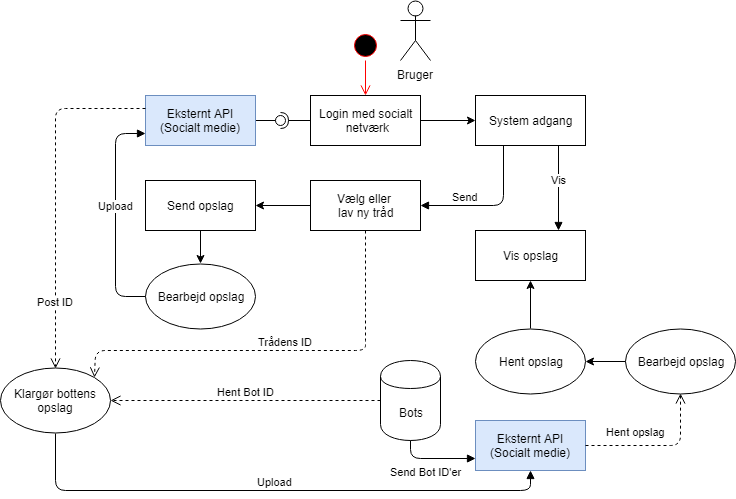
\includegraphics[width=0.8\linewidth]{Projectdoc/Assets/Illustrationer/userbased-system.png}
    \caption{UML diagram over et brugerkonto baseret kommunikations system}
    \label{fig:userbased}
\end{figure}

Brugerne logger ind på platformen [Figur \ref{fig:userbased}] ved hjælp af deres egne kontooplysninger til et given socialt medie. Platformen har nu mulighed for at sende den hemmelige besked direkte til brugerens egen konto. Platformen lægger automatisk den hemmelige besked ind i den pågældende bruger's opslag, og returnere samtidigt opslagets unikke ID tilbage. Dette ID bliver sammen med et unikt tråd ID lageret på en bot. Tråd ID bliver enten generet på stedet, hvis der oprettes en helt ny tråd, eller så bliver et tråd ID nedarvet fra et tidligere ID. Botten har også en konto på det givne sociale medie, kontrolleret af platformen selv. 

Når brugerne af platformen ønsker at få alle opslag vist, så henter systemet alle bots oplag i den rækkefølge som opslagene er tilsendt til botten. Botten har, som før nævnt, gemt data i disse opslag som: tråd struktur og adressen (PostID'et) på beskeden. Det ekstraheret postID kan nu spores tilbage til den bruger der ejer den hemmelige besked.
\\\\
\textit{Fordele:}
\begin{itemize}
    \item[+] \textbf{Brugerkonti som proxy} \hfill \\ 
    Hvis en bot bliver undersøgt vil beskederne ikke umiddelbart kunne blive aflæst. Samtidig vil det også være muligt for en bruger at genskabe deres opslag ved en eventuel nedlukning af en bot.
    \item[+] \textbf{Sammenkædning af posts af samme forfatter} \hfill \\ 
    Med et system som dette hvor opslag hentes fra brugerne selv, kan man samtidig hente og hashe brugerens ID, sådan måde at det ikke kan linkes tilbage til brugeren sig, men indikere at den samme bruger står bag flere opslag.
\end{itemize}
\\
\textit{Ulemper:}
\begin{itemize}
    \item[-] \textbf{Skjul af metadata} \hfill \\
    Denne løsning kræver at en rækker ID'er bliver skjult i metadata på sådan vis at det er genkendeligt for systemet, men ikke mennesker. Et problem der på nuværrende tidspunkt ikke har en løsning.
    \item[-] \textbf{Dobbelt forspørgelse} \hfill \\
    Systemet skal foruden kontakte systems egne bot konti også kontakt den enkelte bruger der opbevare et opslag.
    \item[-] \textbf{Begrænset kontrol over opslag} \hfill \\ 
    Brugeren kan slette deres opslag udenom systemet, og ødelægge trådes struktur.
\end{itemize}